\documentclass[tikz,border=10pt]{standalone}
\usetikzlibrary{arrows.meta, positioning, shapes.geometric}

\begin{document}
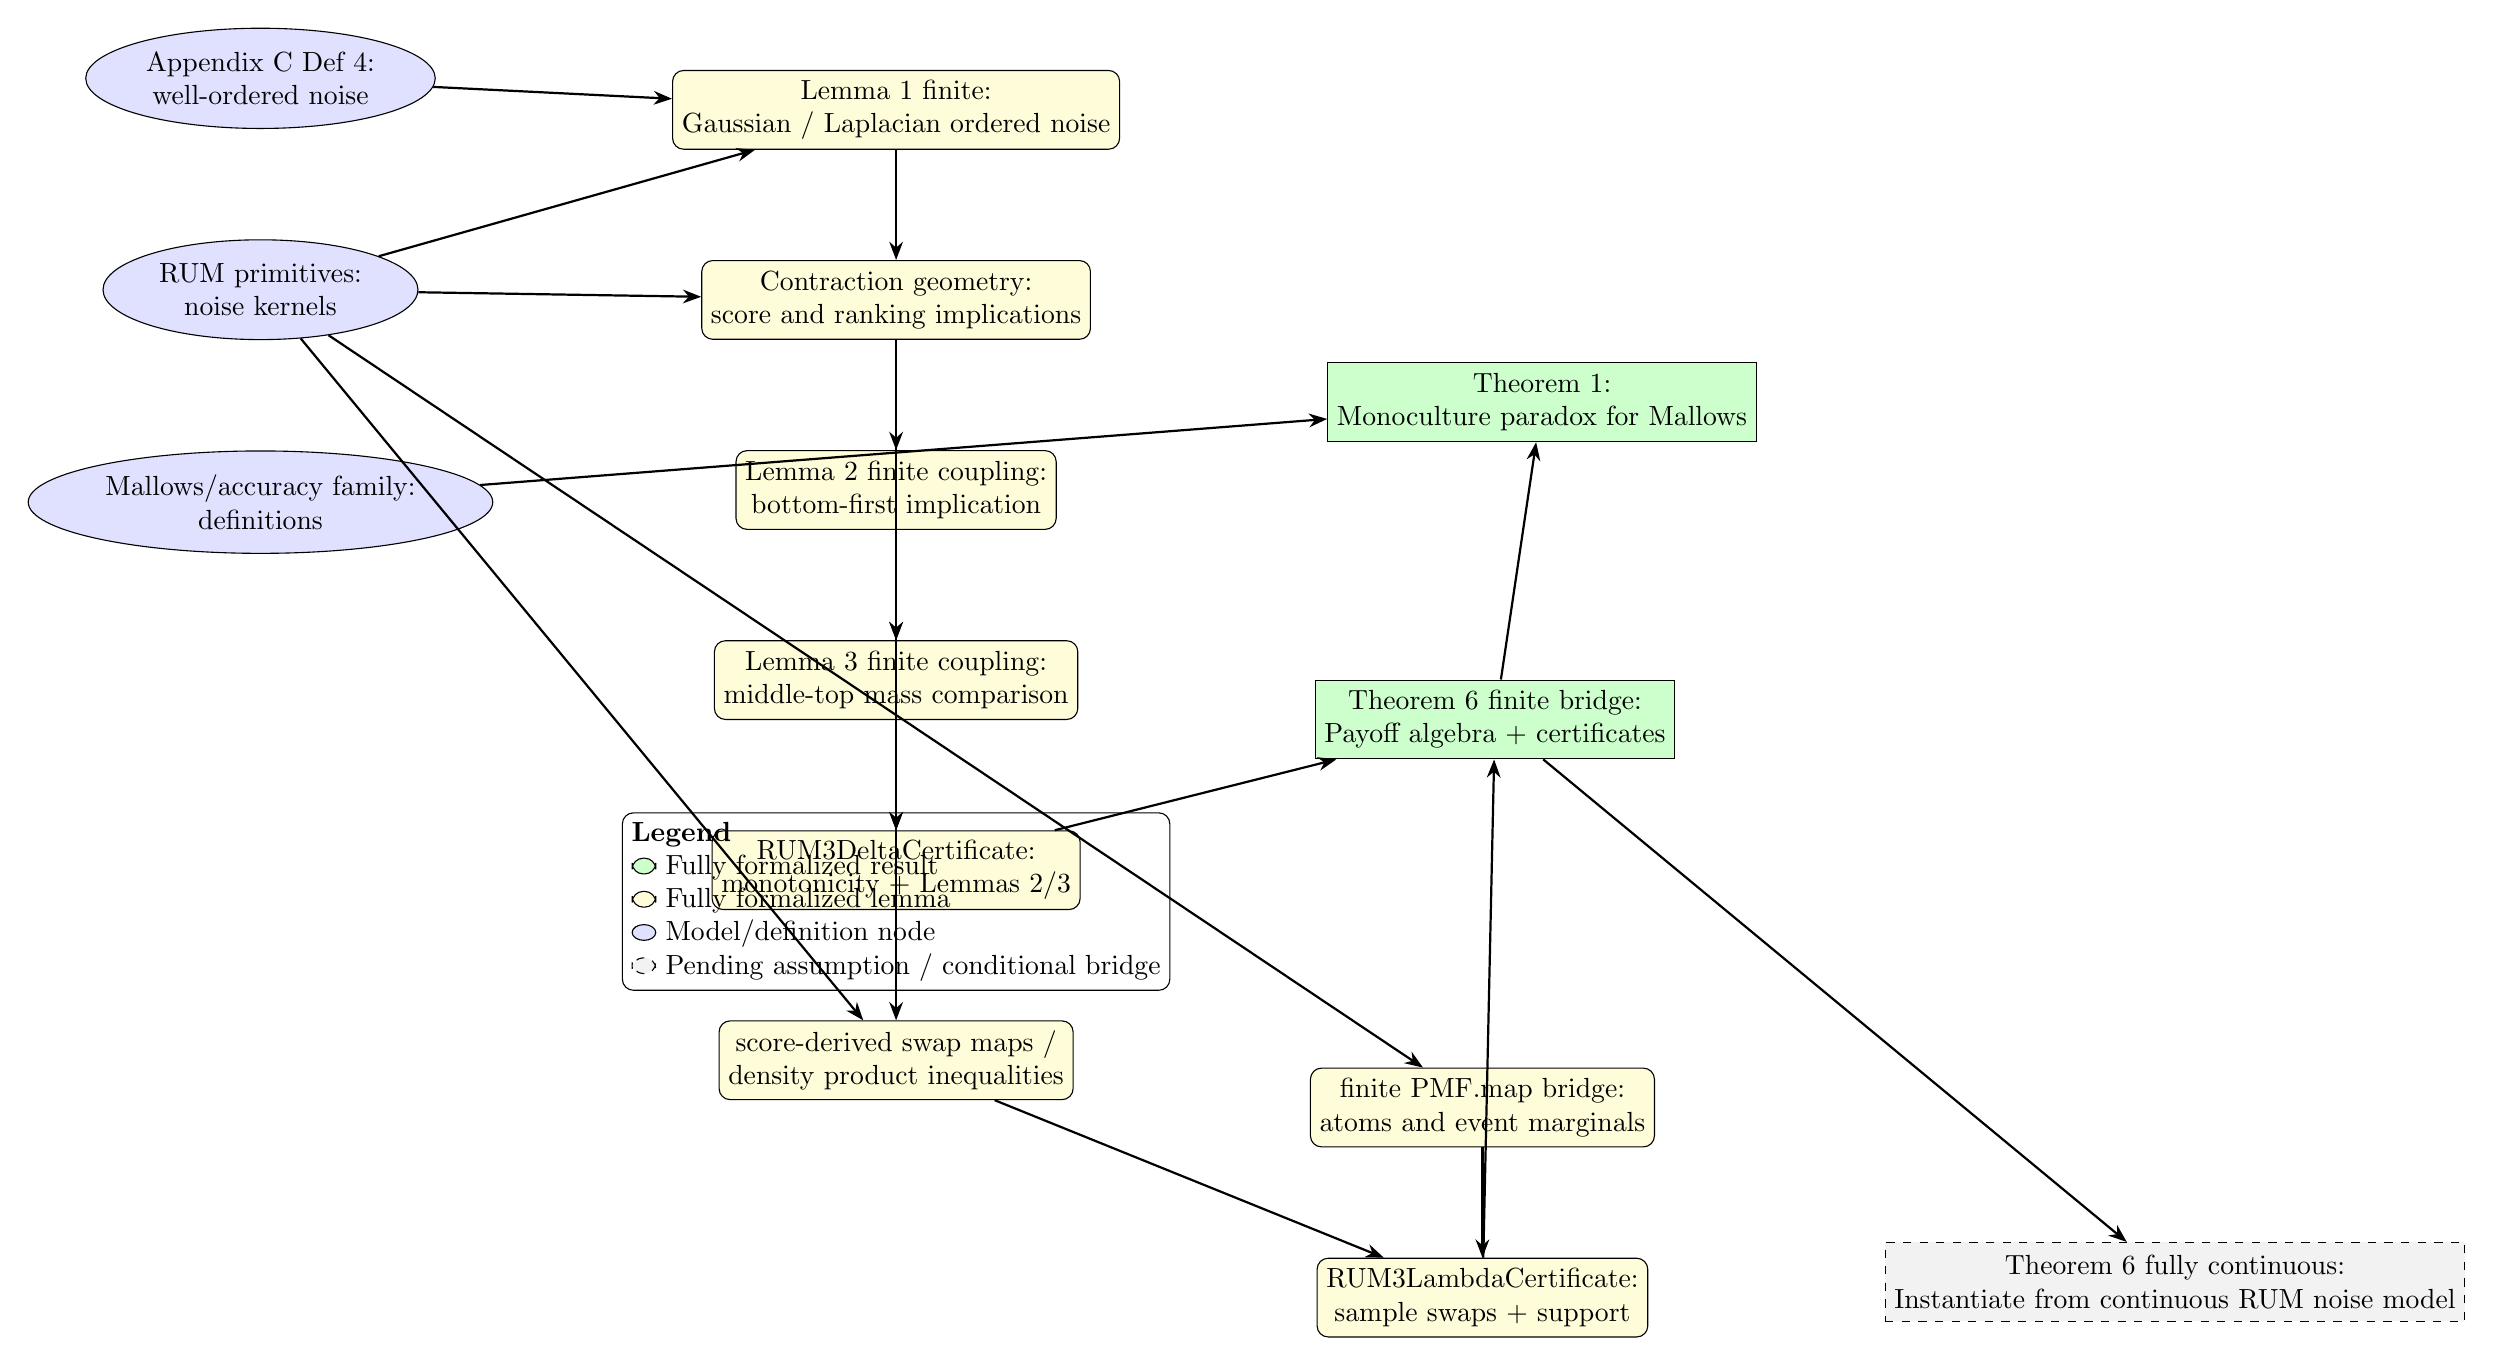
\begin{tikzpicture}[
  node distance=1.4cm and 2.1cm,
  result/.style={rectangle, draw, fill=green!20, minimum width=4cm, minimum height=1cm, align=center},
  lemma/.style={rectangle, rounded corners, draw, fill=yellow!15, minimum width=4cm, minimum height=1cm, align=center},
  model/.style={ellipse, draw, fill=blue!12, minimum width=4cm, minimum height=1cm, align=center},
  open/.style={rectangle, draw, dashed, fill=gray!10, minimum width=4.2cm, minimum height=1cm, align=center},
  arrow/.style={-{Stealth}, thick}
]

% Left column: paper/model definitions.
\node[model] (Def4) {Appendix C Def 4:\\well-ordered noise};
\node[model, below=of Def4] (RUMDefs) {RUM primitives:\\noise kernels};
\node[model, below=of RUMDefs] (MallowsDefs) {Mallows/accuracy family:\\definitions};

% Middle column: formalized lemmas and certificates.
\node[lemma, right=3cm of Def4, yshift=-0.4cm] (L1) {Lemma 1 finite:\\Gaussian / Laplacian ordered noise};
\node[lemma, below=of L1] (ContractionGeom) {Contraction geometry:\\score and ranking implications};
\node[lemma, below=of ContractionGeom] (Lemma2) {Lemma 2 finite coupling:\\bottom-first implication};
\node[lemma, below=of Lemma2] (Lemma3) {Lemma 3 finite coupling:\\middle-top mass comparison};
\node[lemma, below=of Lemma3] (DeltaCert) {RUM3DeltaCertificate:\\monotonicity + Lemmas 2/3};
\node[lemma, below=of DeltaCert] (SwapGeom) {score-derived swap maps /\\density product inequalities};
\node[lemma, right=3cm of SwapGeom, yshift=-0.6cm] (PreimageBridge) {finite PMF.map bridge:\\atoms and event marginals};
\node[lemma, below=of PreimageBridge] (LambdaCert) {RUM3LambdaCertificate:\\sample swaps + support};

% Right column: theorem-level targets.
\node[result, right=3cm of ContractionGeom, yshift=-1.3cm] (Theorem1) {Theorem 1:\\Monoculture paradox for Mallows};
\node[result, right=3cm of Lemma3, yshift=-0.5cm] (Theorem6A) {Theorem 6 finite bridge:\\Payoff algebra + certificates};
\node[open, right=3cm of LambdaCert, yshift=0.2cm] (Theorem6B)
  {Theorem 6 fully continuous:\\Instantiate from continuous RUM noise model};

% Edges from definitions to lemmas.
\draw[arrow] (Def4) -- (L1);
\draw[arrow] (RUMDefs) -- (L1);
\draw[arrow] (RUMDefs) -- (ContractionGeom);
\draw[arrow] (RUMDefs) -- (SwapGeom);
\draw[arrow] (RUMDefs) -- (PreimageBridge);
\draw[arrow] (PreimageBridge) -- (LambdaCert);
\draw[arrow] (MallowsDefs) -- (Theorem1);

% Edges for finite proof chain.
\draw[arrow] (L1) -- (ContractionGeom);
\draw[arrow] (ContractionGeom) -- (Lemma2);
\draw[arrow] (ContractionGeom) -- (Lemma3);
\draw[arrow] (ContractionGeom) -- (SwapGeom);
\draw[arrow] (Lemma2) -- (Lemma3);
\draw[arrow] (Lemma2) -- (DeltaCert);
\draw[arrow] (Lemma3) -- (DeltaCert);
\draw[arrow] (SwapGeom) -- (LambdaCert);
\draw[arrow] (LambdaCert) -- (Theorem6A);
\draw[arrow] (DeltaCert) -- (Theorem6A);
\draw[arrow] (Theorem6A) -- (Theorem6B);

% Theorem 1 depends on core theorem-6 style machinery as well.
\draw[arrow] (Theorem6A) -- (Theorem1);

% Legend
\node[draw, rectangle, rounded corners, below=of ContractionGeom, yshift=-4.6cm, align=left, anchor=north] (Legend) {
    \textbf{Legend} \\
    \tikz\draw[fill=green!20] (0,0) rectangle (0.3,0.2); Fully formalized result \\
    \tikz\draw[fill=yellow!15, rounded corners] (0,0) rectangle (0.3,0.2); Fully formalized lemma \\
    \tikz\draw[fill=blue!12] (0,0) ellipse (0.15 and 0.1); Model/definition node \\
    \tikz\draw[dashed, fill=gray!10] (0,0) rectangle (0.3,0.2); Pending assumption / conditional bridge
};

\end{tikzpicture}
\end{document}
